% ICDM 2026 OWAD — anonymous conference submission (IEEEtran).
% Named camera-ready twin: paper_en_camera.tex
\documentclass[conference]{IEEEtran}

% Local CTAN vendor copy (IEEEtran.cls symlink in this directory).
\usepackage{cite}
\usepackage{amsmath,amssymb,amsfonts}
\usepackage{booktabs}
\usepackage{graphicx}
\usepackage{url}
\usepackage{xcolor}
\usepackage{microtype}
\usepackage{placeins}
% Prefer packing floats on text pages (helps Figs.~3--6 stay with Results).
\renewcommand{\topfraction}{0.95}
\renewcommand{\bottomfraction}{0.9}
\renewcommand{\textfraction}{0.05}
\renewcommand{\floatpagefraction}{0.85}
\setcounter{topnumber}{5}
\setcounter{bottomnumber}{4}
\setcounter{totalnumber}{8}
\setcounter{dbltopnumber}{4}
\usepackage{tikz}
\usetikzlibrary{arrows.meta,fit}

% XeLaTeX fonts with Cyrillic coverage for RU bib titles (IEEEtran defaults to ptm).
\usepackage{fontspec}
\setmainfont{Liberation Serif}
\setsansfont{Liberation Sans}
\setmonofont{Liberation Mono}

\usepackage[hidelinks]{hyperref}

\graphicspath{{images/}}
\hyphenation{electro-en-ceph-a-lo-gram}

% Triple-blind: anonymize site/affiliation wording inside body_en.tex
\newif\ifOWADAnonymous
\OWADAnonymoustrue

\title{Bayesian Changepoint Detection for Event-Aligned REM Means Near Seismic Events}

% Anonymous submission: no names, affiliations, thanks, or date.
\author{%
\IEEEauthorblockN{Anonymous Authors}
\IEEEauthorblockA{Affiliation withheld for triple-blind review}
}

\begin{document}
\maketitle

\begin{abstract}
We test whether an instrumented, brain-derived REM signal in rats shows a statistical regime-shift anomaly near seismic events, and which features and profile hyperparameters describe that anomaly most coherently. Eight-day event-aligned hypnogram windows (\(n=34\) after day-mask with \(K=6\)) are summarized by daily and half-day REM means under a Bayesian single-changepoint model with marginalized discrete onset \(\tau\). Student-\(t\) and skew-normal likelihoods for mean features yield stable \(\mathbb{E}[\tau]\) distributions concentrated a few days from the event. PSIS-LOO ranks retained profile geometries (\(N\), overlap) and mean likelihoods inside one observation builder. A within-window day-shuffle control on the primary mean arm breaks that mid-window onset consensus across seeds (peak \(\tau\) leaves \(\{6,7\}\) for single-regime edges \(\tau=2\) or \(\tau=8\)), matching a synthetic single-changepoint power check, so the onset is tied to event-aligned day order rather than to a generic eight-day REM stretch. Secondary range checks use IIB@\(0.9\) because ordinary Beta is ill-behaved when min–max–normalized daily range concentrates near one. The result is statistical evidence of an anomaly in a neural sleep signal near seismic events---not visual behavioral proof and not operational earthquake prediction.
\end{abstract}

\begin{IEEEkeywords}
REM sleep, changepoint detection, Bayesian inference, PSIS-LOO, neuroseismology, open-world anomaly detection.
\end{IEEEkeywords}

\section{Introduction}

A complete physical model of earthquake preparation is still lacking \cite{Rodkin2011}. At the same time, a large body of geophysical, geochemical, and related precursor observations has been assembled \cite{Cicerone2009,Conti2021}. Those observations do not by themselves authorize operational earthquake forecasting: critical reviews stress uncertain effect sizes and the risk of over-generalization \cite{Geller1997,Conti2021}. The question addressed here is narrower and statistical: do instrumented physiological time series exhibit a distinguishable anomaly—a timed regime onset—in the neighborhood of a seismic event?

Animals can react to environmental changes that accompany earthquake preparation. Behavioral anomalies before shocks and evolutionary arguments for retained sensitivity have been discussed for decades \cite{Kirschvink2000}; links between environmental shifts and behavior appear in interdisciplinary work \cite{Grant2011}; and a few studies report instrumented animal monitoring near event dates \cite{Yokoi2003}. Such reports motivate looking for physiological markers on a controlled recording site. They do not replace continuous measurement of a concrete biosignal under a fixed experimental protocol.

In rodents, stress and anxiety alter the sleep–wake cycle and the structure of paradoxical (REM) sleep \cite{Rampin1991,Meerlo1997,Palma2000,Sanford2010}. Different stressors produce different sleep-phase shifts \cite{Rampin1991,Meerlo1997,Palma2000}, so REM fraction is only an indirect state marker and cannot substitute for corticosterone assays or behavioral anxiety tests. Interpretation must stay conservative: the object of analysis is a REM-associated change in dynamics, not a proven “earthquake stress” construct.

REM sleep in rats is identifiable from EEG/ECoG spectral features and participates in a strong circadian rhythm \cite{Fang2010,Vyazovskiy2005}. At the study site, hypnograms are obtained by automated staging of continuous recordings \cite{Saevskiy2025}, yielding multivariate REM summaries aligned to seismic events. Classical neuroseismological reports from the same station emphasized the range of the REM profile—often over twelve non-overlapping two-hour bins—and described a pronounced effect roughly two to four days before and after strong events. The present work estimates a different quantity: the onset of a regime change in a Bayesian single-changepoint model with discrete time index \(\tau\) on an eight-day event-relative window. That onset parameter is not identical to the classical window of maximum effect and needs a separate reading. Framed for open-world monitoring, the technical task is changepoint / regime-shift detection in short, heterogeneous multivariate physiological series whose external driver is an irregular seismic context rather than a fully labeled laboratory intervention.

Data constraints dominate the methodological choice. Events of sufficient intensity are rare, so the sample of event–animal pairs is extremely small; daily summaries are autocorrelated \cite{Hyndman2018}; and animals, seasons, and shock parameters are heterogeneous. High-capacity models overfit easily in this regime, and random train–test splits on temporal structures inflate scores through leakage \cite{Bergmeir2012}. A Bayesian single-changepoint formulation with an explicit onset parameter and posterior uncertainty \cite{carlin1992hierarchical,Sinkovec2022} matches the data deficit more closely, provided candidate preprocessing and likelihood configurations are compared by predictive density such as PSIS-LOO \cite{Vehtari2017}.

This paper develops an interpretable Bayesian single-changepoint model for eight-day REM series near seismic events, focusing on mean brain-derived features and profile hyperparameters that yield stable onset posteriors. We treat the result as statistical evidence of a regime-shift anomaly in an instrumented neural sleep signal—not as visual behavioral proof and not as operational earthquake prediction \cite{Geller1997}. Range likelihoods known a priori to destroy \(\tau\) interpretability are excluded from the main analysis. The remainder of the manuscript presents the data, the model, the design, the results, and the limits of interpretation.

\section{Related Work}

Work on earthquake preparation and precursors documents incomplete physical models alongside many geophysical and geochemical observations \cite{Rodkin2011,Cicerone2009,Conti2021}. Critical assessments emphasize that such observations do not establish operational forecasting \cite{Geller1997,Conti2021}. Parallel biological threads describe animal behavioral anomalies before shocks \cite{Kirschvink2000}, possible environmental mediators \cite{Grant2011}, and occasional instrumented monitoring near event dates \cite{Yokoi2003}. That literature supports looking for early biosignal indicators in a controlled setting, but it rarely supplies a statistical estimand for the \emph{onset} of a physiological regime change on continuous recordings.

Stress and anxiety reshape rodent sleep, including paradoxical (REM) sleep, in a stressor-dependent way \cite{Rampin1991,Meerlo1997,Palma2000,Sanford2010}. Spectral EEG/ECoG features make REM identifiable within a strong circadian structure \cite{Fang2010,Vyazovskiy2005}, and automated staging yields continuous hypnograms suitable for event-aligned analysis \cite{Saevskiy2025}. Classical neuroseismological reports from the same recording site focused on the range of the REM profile and described effects concentrated roughly two to four days around strong events. Those reports motivate REM as a biosignal, yet they leave open how to time a regime onset under posterior uncertainty when samples are tiny and heterogeneous.

Changepoint detection treats abrupt transitions in time-series dynamics as a core mining problem, with surveys spanning supervised and unsupervised families across monitoring domains \cite{Aminikhanghahi2017}. Bayesian formulations provide retrospective hierarchical analyses \cite{carlin1992hierarchical} and online run-length inference for regime shifts \cite{Adams2007}. In short autocorrelated series \cite{Hyndman2018}, random validation splits can leak temporal structure \cite{Bergmeir2012}, so small-sample settings favor models that expose uncertainty \cite{Sinkovec2022} and compare predictive fit via tools such as PSIS-LOO \cite{Vehtari2017}. High-capacity anomaly detectors are less attractive when event–animal pairs are scarce and external seismic context is irregular rather than fully labeled.

This paper sits at that intersection. We cast event-aligned multivariate REM windows as a single-changepoint task for detecting a seismic-event-associated anomaly in a brain-derived sleep signal, emphasizing mean features and profile hyperparameters that yield interpretable \(\mathbb{E}[\tau]\) distributions under Student-\(t\) or skew-normal likelihoods. Range families known a priori to destroy onset interpretability are excluded from the main narrative. The study does not claim operational earthquake prediction \cite{Geller1997} and does not measure stress with independent biomarkers.

\section{Data}

Continuous bioelectric recordings were collected at the Institute station of the Kamchatka Branch of the Geophysical Survey of the Russian Academy of Sciences (Petropavlovsk-Kamchatsky). Subjects were adult male Passyuk rats weighing 200–250 g, housed individually at \(23\pm 1^{\circ}\)C under a fixed 12 h light / 12 h dark cycle with free access to food and water. All procedures were approved by the bioethics committee of Southern Federal University.

Sleep–wake states were assessed from electrical activity of the sensorimotor cortex (ECoG) and hippocampal field CA1. Electrodes were implanted under anesthesia, and recording began no earlier than one week after surgery. Signals were digitized at 1 kHz (PBX2/32sp-r/32fp300 amplifier; L-ACRD E~14-440 ADC) and exported daily to object storage. Hypnograms were produced by an automated staging pipeline of the SFU Neurotechnology Research Center—a simplified version of the method in \cite{Saevskiy2025}. Each daily recording was split into non-overlapping 5 s epochs; high-amplitude artifact epochs were removed. Slow-wave sleep was labeled from ECoG power in the delta band (2.5–5.5 Hz) \cite{Fang2010}. Paradoxical (REM) sleep was marked by a high hippocampal theta/delta ratio (theta 5.5–8 Hz) \cite{Fang2010,Saevskiy2025}. Remaining epochs were assigned to wakefulness. The output is a sequence of wake / SWS / REM labels from which daily REM profiles are constructed; profile parameters are defined in the Methods section.

The base sample comprises 14 seismic event dates from 2022–2025. Inclusion required instrumental intensity at the station greater than 2 (peak accelerations after 0.1–10 Hz filtering following \cite{GOST2017}) and a continuous hypnogram for eight days before and eight days after the shock. Station coordinates are \(53.06^{\circ}\)N, \(158.61^{\circ}\)E. On 2025-07-02 and 2025-07-20, four animals (R1–R4) were recorded concurrently, yielding multiple event–animal pairs on the same date. Analysis uses eight-day windows relative to the event date. The pre-event window forms the primary pre-shock series. When needed, the post-event window is time-reversed (\texttt{after\_reversed}) so that it can enter the same feature pipeline; biologically that series is closer to a recovery period and may differ in quality from the pre-event window. Incomplete days without a hypnogram and pre-specified artifact days are masked as NaN and skipped in the likelihood; a window remains in the sample if at least six days are valid. After masking, the primary cohort contains 34 windows. The resulting objects are short, heterogeneous, multivariate event-aligned REM series derived from brain recordings—the input for detecting a changepoint-style anomaly associated with the seismic event. Feature construction and the screening grid are described next.

\section{Method}

Daily REM profiles are built from the hypnogram as the fraction of time spent in paradoxical sleep in successive temporal bins. A profile is parameterized by the number of bins per day \(N\) and the overlap fraction \(\mathrm{ov}\) of adjacent windows; the classical twelve non-overlapping two-hour bins correspond to \((N,\mathrm{ov})=(12,0)\). From a day profile \(P=(p_1,\ldots,p_N)\) we compute the mean \(\bar P=N^{-1}\sum_i p_i\) and, when needed for secondary checks, the range \(R=\max_i p_i-\min_i p_i\), including half-day (light/dark) versions of the same summaries. Mean and range are two separate scalar features, not a sum: when both are active they share one common \(\tau\). The primary analysis uses mean features, which after window-wise scaling to \([-1,1]\) yield real-valued series with stable onset posteriors. Artifact days and days without a hypnogram are masked as NaN and skipped in the likelihood without imputation and without shrinking the discrete grid of \(\tau\). A window enters the sample if at least \(K=6\) days remain valid.

For a feature vector \(\mathbf{x}_t\) on days \(t=1,\ldots,8\) we use a single regime switch

\begin{equation*}
\mathbf{x}_t \sim
\begin{cases}
p(\mathbf{x}_t\mid\boldsymbol{\theta}_1), & t < \tau,\\
p(\mathbf{x}_t\mid\boldsymbol{\theta}_2), & t \ge \tau.
\end{cases}
\end{equation*}

The discrete day index is event-aligned so that \(t=8\) is the day nearest the shock (one day from the event) and \(t=1\) is eight days from the event; calendar distance in days is \(9-t\). The discrete onset \(\tau\) is given a uniform prior on \(\mathcal{T}=\{2,\ldots,8\}\) and is marginalized for NUTS sampling \cite{HoffmanGelman2014},

\begin{equation*}
p(\mathbf{y}\mid\boldsymbol{\theta})
=
\frac{1}{|\mathcal{T}|}
\sum_{k\in\mathcal{T}}
p(\mathbf{y}\mid\tau{=}k,\boldsymbol{\theta}).
\end{equation*}


\begin{figure*}[t]
  \centering
  \resizebox{0.78\textwidth}{!}{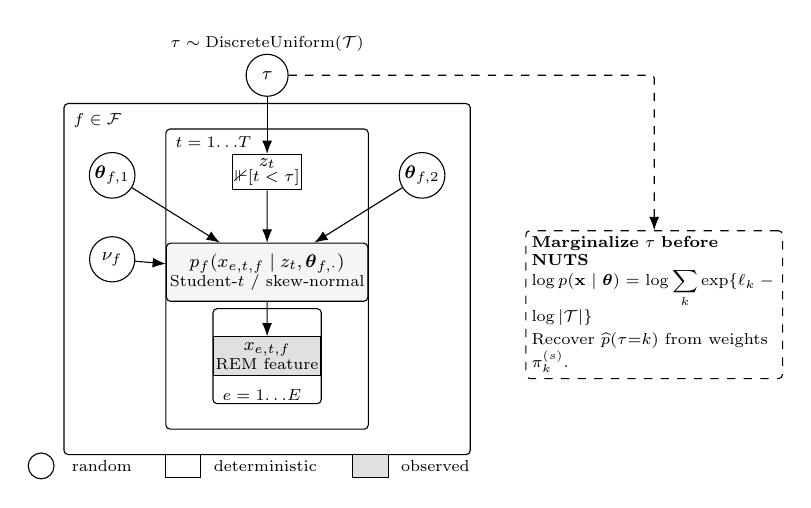
\begin{tikzpicture}[
  >=Latex,
  scale=0.82, every node/.style={transform shape, font=\footnotesize},
  latent/.style={circle, draw, minimum size=7mm, align=center, inner sep=1pt},
  deterministic/.style={rectangle, draw, minimum width=10mm, minimum height=5.5mm,
    align=center, inner sep=1pt},
  observed/.style={rectangle, draw, fill=black!12, minimum width=15mm,
    minimum height=6mm, align=center, inner sep=1pt},
  likelihood/.style={rounded corners=1.5pt, draw, fill=black!4, minimum width=24mm,
    minimum height=9mm, align=center, inner sep=1.5pt},
  annotation/.style={rectangle, draw, dashed, rounded corners=1.5pt, align=left,
    inner sep=2.5pt, font=\scriptsize},
  plate/.style={draw, rounded corners=1.5pt, inner sep=3.5pt}
]
  \node[latent, minimum size=6.5mm] (tau) at (0, 2.7) {$\tau$};
  \node[font=\scriptsize, anchor=south] at (0, 2.95)
    {$\tau\sim\mathrm{DiscreteUniform}(\mathcal T)$};
  \node[deterministic] (z) at (0, 1.2) {$z_t$\\[-3pt]\scriptsize $\mathbb{1}[t<\tau]$};
  \node[latent] (theta1) at (-2.4, 1.15) {$\boldsymbol{\theta}_{f,1}$};
  \node[latent] (theta2) at (2.4, 1.15) {$\boldsymbol{\theta}_{f,2}$};
  \node[latent] (nu) at (-2.4, -0.15) {$\nu_f$};
  \node[likelihood] (lik) at (0, -0.35) {$p_f(x_{e,t,f}\mid z_t,\boldsymbol{\theta}_{f,\cdot})$\\[-1pt]
    \scriptsize Student-$t$ / skew-normal};
  \node[observed] (x) at (0, -1.65) {$x_{e,t,f}$\\[-1pt]\scriptsize REM feature};

  \draw[->] (tau) -- (z);
  \draw[->] (z) -- (lik);
  \draw[->] (theta1) -- (lik);
  \draw[->] (theta2) -- (lik);
  \draw[->] (nu) -- (lik);
  \draw[->] (lik) -- (x);

  \node[plate, fit=(x), inner xsep=0pt, inner ysep=10pt] (eventplate) {};
  \node[plate, fit=(z) (lik) (eventplate), inner xsep=0pt, inner ysep=9pt] (timeplate) {};
  \node[plate, fit=(theta1) (theta2) (nu) (timeplate), inner sep=9pt] (featureplate) {};
  \node[font=\scriptsize, anchor=north west, xshift=1pt, yshift=-1pt]
    at (featureplate.north west) {$f\in\mathcal F$};
  \node[font=\scriptsize, anchor=north west, xshift=1pt]
    at (timeplate.north west) {$t=1{\ldots}T$};
  \node[font=\scriptsize, anchor=south west, xshift=1pt, yshift=-2pt]
    at (eventplate.south west) {$e=1{\ldots}E$};

  \node[annotation, anchor=north west, text width=38mm] (marg) at (4.0, 0.3) {
    \textbf{Marginalize $\tau$ before NUTS}\\[1pt]
    $\displaystyle \log p(\mathbf{x}\mid\boldsymbol{\theta})
      =\log\sum_{k}\exp\{\ell_k-\log|\mathcal T|\}$\\[2pt]
    Recover $\widehat p(\tau{=}k)$ from weights $\pi_k^{(s)}$.
  };
  \draw[->, dashed, rounded corners=1pt]
    (tau.east) -- (tau.east -| marg.north) -- (marg.north);

  \node[latent, minimum size=4mm] (legendlatent) at (-3.5, -3.35) {};
  \node[anchor=west, font=\scriptsize] at (-3.15, -3.35) {random};
  \node[deterministic, minimum width=5.5mm, minimum height=3.5mm] (legenddet) at (-1.3, -3.35) {};
  \node[anchor=west, font=\scriptsize] at (-0.95, -3.35) {deterministic};
  \node[observed, minimum width=5.5mm, minimum height=3.5mm] (legendobs) at (1.6, -3.35) {};
  \node[anchor=west, font=\scriptsize] at (1.95, -3.35) {observed};
\end{tikzpicture}
}
  \caption{Probabilistic plate diagram of the Bayesian single-changepoint model.
  Circles are random variables; $z_t$ is a deterministic regime indicator; the shaded box is observed data.
  The dashed box marks analytic marginalization of discrete $\tau$ before NUTS.}
  \label{fig:tau-model}
\end{figure*}


The posterior \(p(\tau{=}k\mid\mathbf{y})\) and \(\mathbb{E}[\tau\mid\mathbf{y}]\) are recovered from posterior draws of \(\boldsymbol{\theta}\). When several features are active in one configuration, they share a common \(\tau\). Figure~\ref{fig:tau-model} shows the probabilistic plate diagram: a discrete uniform prior on \(\tau\), a deterministic regime indicator \(z_t=\mathbb{1}[t<\tau]\), feature-wise likelihoods, and analytic marginalization of \(\tau\) before NUTS. This construction tests for a seismic-event-associated anomaly as a changepoint in short brain-derived REM summaries—an instrumented physiological signal rather than a visual behavioral report.

Likelihoods are restricted a priori to families that match the support of the feature and that are known not to destroy interpretability of \(\tau\). For mean features we use Student-\(t\), which accommodates heavier tails and a few outlying days, and skew-normal, which allows asymmetry in the day-to-day distribution of means. Both keep \(\mathbb{E}[\tau]\) away from pathological prior-edge pile-ups on mean-only series. Classical site reports emphasized profile range, but several unit-interval Beta specifications for range are known in advance to place unusable mass of \(\mathbb{E}[\tau]\) at the far end of the prior grid or to inflate predictive scores through boundary density. Those families are excluded from the main analysis rather than advertised as competing “winners.” When a range feature is retained for a secondary check, we use only an interval-inflated Beta (IIB@\(0.9\)) motivated by the fact that, with few bins and min–max normalization over the eight-day window, daily range often lies near one.

Generalization among retained configurations is scored by PSIS-LOO \cite{Vehtari2017}, with the observation unit equal to an event–animal pair and a normalized score \(\overline{\mathrm{elpd}}/(F\cdot E')\) inside a fixed observation builder (day mask on, \(K=6\)). LOO ranks profile geometry and mean likelihood choices; it is not used to rehabilitate a priori inadequate range families. Windows flagged as influential by Pareto-\(\hat k\) are reported by ID and are not deleted. Sampling uses NUTS under the marginalized \(\tau\) model; we monitor \(\hat R\), effective sample size, and Pareto-\(\hat k\). The combinatorial grid over profile geometry is specified next.

\section{Experimental Setup}

The design asks which profile geometries and mean likelihoods yield a stable, interpretable onset for an event-associated REM anomaly on the same eight-day windows. An exhaustive grid varies \(N\in\{12,24\}\), \(\mathrm{ov}\in\{0,0.25,0.5\}\), and feature blocks from \texttt{daily} / \texttt{day} / \texttt{night} summaries, with at most three blocks active. Mean likelihoods are Student-\(t\) and skew-normal. Range likelihood families known a priori to produce unusable \(\tau\) posteriors are omitted from the main ranking; when range is included as a secondary check, only IIB@\(0.9\) is retained. The discrete onset lies on \(\tau\in\{2,\ldots,8\}\) and is marginalized under NUTS. All fits use day-mask on with \(K=6\), nan-padding export, and a shared screening MCMC budget (tune \(1000\), draws \(500\), two chains). The completed table contains \(1548\) successful configurations; the primary interpretive slice is the mean-only subset (\(n=84\)), with jointly active mean-and-range IIB cells used only as a secondary contrast.

Ranking among retained cells uses \(\overline{\mathrm{elpd}}/(F\cdot E')\) inside one builder. We report \(\mathbb{E}[\tau]\) distributions for Student-\(t\) versus skew-normal, the corresponding calendar distance \(9-\tau\), and profile hyperparameters (\(N\), overlap, daily versus half-day blocks) that concentrate posterior mass in a coherent mid-window band. Confirmatory refits on the primary cohort of \(34\) windows probe day-mask sensitivity (mask off, before-only). On the primary mean Student-\(t\) arm (\texttt{daily:mean}, \(N=24\), \(\mathrm{ov}=0\)), a within-window day-shuffle control permutes valid days independently inside each window while keeping NaN masks fixed (seeds \(0,1,2\); confirmatory MCMC budget matched to the real-date fit). Influential windows are reported by Pareto-\(\hat k\) ID and never silently dropped.

\section{Results}

After day-mask with \(K=6\), the primary cohort contains \(34\) windows. The interpretive center of the study is whether a regime-shift anomaly appears in brain-derived REM summaries near seismic events, and which mean features and profile hyperparameters describe that onset most coherently.

\subsection{Mean features: stable onset distributions}

Mean-only configurations (\(n=84\)) yield \(\mathbb{E}[\tau]\approx 5.78\) (median \(5.80\)) with a \(0\%\) rate of pile-up at the far prior edge \(\tau=2\). On the event-aligned index this corresponds to an onset about three days from the event (\(9-\tau\)). Both Student-\(t\) (\(n=42\); median \(\mathbb{E}[\tau]=5.64\)) and skew-normal (\(n=42\); median \(6.25\)) produce compact, well-behaved histograms without the pathological floor mass that disqualifies several range families a priori (Fig.~\ref{fig:mean-only}). Skew-normal shifts the onset slightly closer to the event than Student-\(t\) (about \(+0.42\) on paired cells), while remaining inside the same multi-day band. These distributions are the main empirical support for a statistical anomaly in the REM signal: the posterior mean onset is neither pinned to an unusable prior edge nor scattered uniformly across the window.

Within the mean slice, LOO ranks profile geometry and likelihood choice. Table~\ref{tab:loo-topk} lists the top-10 mean-only cells by \(\overline{\mathrm{elpd}}/(F\cdot E')\): denser daily profiles with \(N=24\) and low overlap lead, with Student-\(t\) and skew-normal nearly tied at the top, and mid-window \(\mathbb{E}[\tau]\) throughout. Higher elpd among retained mean cells tends to accompany mid-window \(\mathbb{E}[\tau]\) rather than edge artifacts. Half-day (\texttt{day} / \texttt{night}) blocks and the classical \((N,\mathrm{ov})=(12,0)\) versus denser \(N=24\) profiles change the concentration of \(\mathbb{E}[\tau]\) only modestly once the mean feature and a heavy-tailed or skew observation model are fixed (Fig.~\ref{fig:mean-profile})—evidence that the anomaly is not an artifact of a single binning recipe.

% Auto-generated by figures/make_loo_topk_table.py — do not edit by hand.
\begin{table}[t]
  \centering
  \caption{Top-10 mean-only cells by $\overline{\mathrm{elpd}}/(F\cdot E')$ ($n=84$).}
  \label{tab:loo-topk}
  \setlength{\tabcolsep}{3.5pt}
  \renewcommand{\arraystretch}{1.05}
  \begin{tabular}{@{}r l l r r r r r@{}}
    \toprule
    \# & features & lik & $N$ & ov &
    $\overline{\mathrm{elpd}}$ & $\mathbb{E}[\tau]$ & $\hat k_{\max}$ \\
    \midrule
    1 & \texttt{daily} & Student-$t$ & 24 & 0 & 0.480 & 6.03 & 0.67 \\
    2 & \texttt{daily} & skew-normal & 24 & 0 & 0.476 & 6.14 & 1.08 \\
    3 & \texttt{daily} & Student-$t$ & 24 & 0.25 & 0.342 & 6.15 & 0.73 \\
    4 & \texttt{daily} & skew-normal & 24 & 0.25 & 0.338 & 6.43 & 0.82 \\
    5 & \texttt{daily} & skew-normal & 24 & 0.50 & 0.281 & 6.32 & 0.60 \\
    6 & \texttt{daily} & Student-$t$ & 24 & 0.50 & 0.279 & 5.57 & 0.65 \\
    7 & \texttt{daily+night} & skew-normal & 24 & 0 & 0.276 & 6.38 & 1.03 \\
    8 & \texttt{daily+night} & Student-$t$ & 24 & 0 & 0.276 & 5.88 & 0.57 \\
    9 & \texttt{daily} & Student-$t$ & 12 & 0 & 0.244 & 5.71 & 0.39 \\
    10 & \texttt{daily} & skew-normal & 12 & 0 & 0.243 & 6.22 & 0.78 \\
    \bottomrule
  \end{tabular}
\end{table}


\begin{figure*}[!t]
  \centering
  
\includegraphics[width=0.88\textwidth]{fig_mean_only_by_lik}
  \caption{Mean-only configurations: histograms of $\mathbb{E}[\tau]$ under Student-$t$ and skew-normal.}
  \label{fig:mean-only}
\end{figure*}

\begin{figure*}[!t]
  \centering
  \includegraphics[width=0.88\textwidth]{fig_mean_by_profile}
  \caption{Mean-only onset versus profile hyperparameters $N$ and overlap (mean $\pm$ std of $\mathbb{E}[\tau]$).}
  \label{fig:mean-profile}
\end{figure*}

\FloatBarrier

\subsection{Confirmatory mean diagnostics}

A long confirmatory Student-\(t\) refit on the top mean-only cell (\texttt{daily:mean}, \(N=24\), \(\mathrm{ov}=0\); Table~\ref{tab:loo-topk}, rank~1) sharpens what the grid-level \(\mathbb{E}[\tau]\) summaries leave implicit. Posterior median predictive densities with a \(90\%\) band separate the before/after regimes more clearly than a mean-parameter plug-in curve: the bulk of the day-to-day mean stays nearly fixed, while the anomaly shows up in the tails and in the onset posterior (MAP \(\tau=7\), \(\mathbb{E}[\tau]\approx 5.74\) under shared \(\nu\)). Allowing separate degrees of freedom per regime on the same cell moves \(\mathbb{E}[\tau]\) only slightly (\(\approx 6.01\)) and leaves \(\mu\) almost unchanged, but shrinks the \(\sigma\)-gap and yields \(\nu_2\approx 13<\nu_1\approx 30\)---heavier tails after the MAP onset (Fig.~\ref{fig:diag-mean-nu}). That \(\nu\)-split is a confirmatory check, not part of the primary LOO ranking.

\begin{figure}[!t]
  \centering
  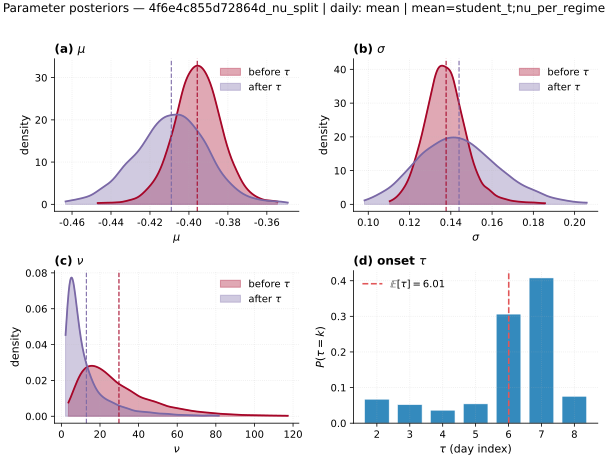
\includegraphics[width=\columnwidth]{fig_diag_mean_nu_params}\\[0.35em]
  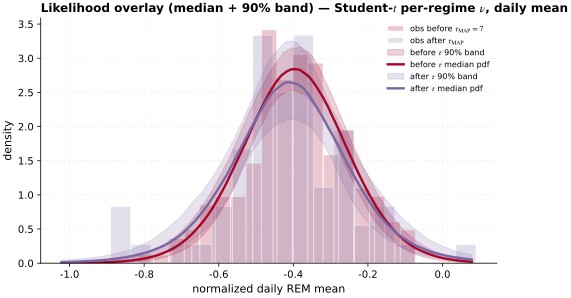
\includegraphics[width=\columnwidth]{fig_diag_mean_nu_overlay}
  \caption{Confirmatory Student-$t$ with per-regime $\nu$ on \texttt{daily:mean} ($N=24$, $\mathrm{ov}=0$): before/after parameter posteriors (top) and median predictive density with $90\%$ band (bottom).}
  \label{fig:diag-mean-nu}
\end{figure}

\FloatBarrier

\subsection{Interpretation}

Taken together, the mean-based fits support a concrete reading. Instrumented hypnograms—not visual behavioral watching—carry a changepoint-style anomaly in REM dynamics aligned to seismic events. The most plausible descriptions in the retained grid combine a daily (or half-day) mean REM feature with Student-\(t\) or skew-normal noise and profile hyperparameters in the screened \(N\times\mathrm{ov}\) set; under those choices, \(\mathbb{E}[\tau]\) concentrates a few days from the event with posterior uncertainty summarized by HDI width on the order of one to two index days. That is a statistical confirmation of an anomaly and a ranking of descriptive configurations, not a causal proof that the earthquake produced the physiological shift, and---given the within-window control below---not a claim that event-aligned day order alone uniquely produces the onset peak.

\subsection{Within-window day-shuffle control}

To test whether the mid-window onset peak requires the observed order of days inside each event-aligned window, we permute finite day observations independently within each window on the primary confirmatory Student-\(t\) cell, leaving NaN masks in place and without reassigning windows across event dates. Averaged over seeds \(0\)--\(2\) at the same confirmatory MCMC budget as the real-date fit, mean \(p(\tau=k)\) does \emph{not} become approximately uniform on \(\mathcal{T}=\{2,\ldots,8\}\): mass still peaks near \(\tau=7\) (about \(0.42\)), and the mean absolute deviation from \(1/|\mathcal{T}|\) remains comparable to the real fit (about \(0.082\) versus \(0.086\); Fig.~\ref{fig:null-within-window}). The real series retains concentration at \(\tau=6\)--\(7\). Because within-window permutation fails to flatten the PMF, the onset pattern is not uniquely explained by event-aligned day order alone; residual mid/late-window structure under the null keeps ordering and causal readings cautious.

\begin{figure}[!t]
  \centering
  
\includegraphics[width=\columnwidth]{fig_null_within_window}
  \caption{Within-window day-shuffle control on the primary mean Student-$t$ arm: mean $p(\tau=k)$ for the real series versus the average over shuffle seeds $0$--$2$. Dashed line: uniform $1/|\mathcal{T}|$ on $\{2,\ldots,8\}$. Shuffle retains residual mass near $\tau=7$ rather than flattening.}
  \label{fig:null-within-window}
\end{figure}

\FloatBarrier

\subsection{Secondary checks}

When a range feature is added under the only retained range likelihood (IIB), jointly active mean-and-range cells remain free of floor pile-up and place \(\mathbb{E}[\tau]\) in a similar multi-day band (IIB mean+range median about \(5.7\)). A confirmatory IIB range-only refit (\(N=12\), \(\mathrm{ov}=0\); observations scaled as \(y=\mathrm{range}/2\)) with \(\tau_{\mathrm{MAP}}=7\) makes the unit-interval pattern explicit (Fig.~\ref{fig:diag-iib}): before the MAP onset, median \(y\approx 0.74\) with \(20.7\%\) of day-observations at \(y\ge 0.9\) (and \(5.6\%\) pinned at the ceiling \(y=1\)); after, median \(y\approx 0.70\) with only \(12.1\%\) at \(y\ge 0.9\) (\(1.5\%\) at one). Event-wise, median(after)\(<\)median(before) in \(20/33\) windows. Mask-off and before-only confirmatory runs on \(n=34\) move \(\mathbb{E}[\tau]\) farther from the event, showing sensitivity to the observation builder. These checks bound interpretation; they are not the primary evidence story.

\begin{figure}[!t]
  \centering
  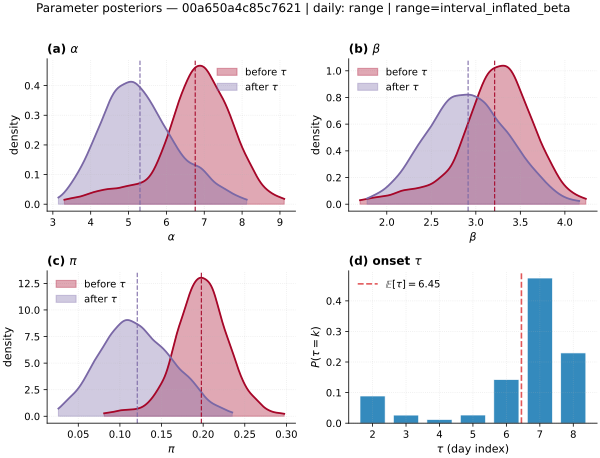
\includegraphics[width=\columnwidth]{fig_diag_iib_params}\\[0.35em]
  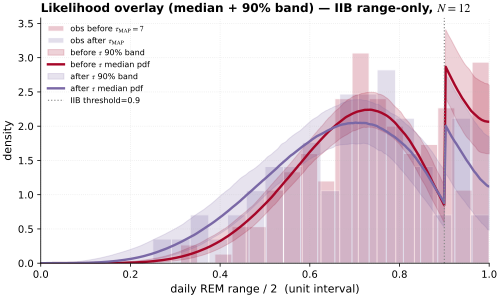
\includegraphics[width=\columnwidth]{fig_diag_iib_overlay}
  \caption{Confirmatory IIB range-only cell ($N=12$, $\mathrm{ov}=0$; $y=\mathrm{range}/2$): before/after parameter posteriors (top) and median predictive density with $90\%$ band (bottom).}
  \label{fig:diag-iib}
\end{figure}

\FloatBarrier

\section{Discussion and Limitations}

The central reading is interpretive. Continuous ECoG-based hypnograms provide a brain-derived REM signal in which a single-changepoint model finds a coherent regime-shift anomaly near seismic events. That confirmation is statistical and instrumented: it does not rest on visual watching of animal behavior, and it does not equate REM change with a measured stress hormone response. Under mean features with Student-\(t\) or skew-normal likelihoods, posterior means \(\mathbb{E}[\tau]\) concentrate a few days from the event and avoid pathological prior-edge pile-ups. The grid then ranks which profile hyperparameters—bin count \(N\), overlap, daily versus half-day blocks—and which of the two mean likelihoods describe that anomaly most coherently by predictive density inside one builder. In that sense the contribution is both a detection claim (a coherent mid-window onset under retained mean specs) and a descriptive claim (these features and hyperparameters are the most plausible among the retained set), tempered by the failed within-window uniformity null below.

We deliberately de-emphasize range likelihood families that were known a priori to yield unusable onset posteriors. Classical reports at the site used profile range as a summary, but several Beta-type range models pull \(\mathbb{E}[\tau]\) to the far prior edge or inflate elpd through boundary density. Advertising those families as LOO “winners” would confuse predictive score with interpretability. Retaining only IIB for secondary range checks, and centering the narrative on mean distributions, keeps the manuscript aligned with the scientific target: an interpretable brain-signal anomaly, not a bake-off among discarded specifications.

Mean and range therefore invite different readings of the same windows. Under mean Student-\(t\), the location bulk barely moves and the regime contrast lives in tails, scale, and \(\tau\); the confirmatory \(\nu\)-split sharpens that story (\(\nu_2<\nu_1\)) without changing the primary ranking. Under IIB range, the readable signal is a pre-onset ceiling near one that thins after \(\tau_{\mathrm{MAP}}\), not a large shift of the central tendency. Both views are consistent with a mid-window onset a few days from the event, but they are not interchangeable summaries of “the” REM anomaly. Limits of that confirmatory layer are deliberate: one shared-\(\nu\) cell, one \(\nu\)-split sibling, and one IIB range refit---useful diagnostics, not a fresh grid.

The estimand remains an onset inside an eight-day window, not the classical two-to-four-day effect window for REM-profile range. Larger \(\tau\) is closer to the shock on the event-aligned index. Day-mask and stratum choices move \(\mathbb{E}[\tau]\). The within-window day-shuffle control fails to drive mean \(p(\tau=k)\) to uniformity and leaves residual mid/late-window mass (Fig.~\ref{fig:null-within-window}), so the pattern is not uniquely tied to event-aligned day order and causal attribution to the earthquake calendar stays weak. Limits include the small cohort (\(n=34\)), the single-changepoint assumption, the absence of independent stress biomarkers, and the lack of an operational forecasting claim \cite{Geller1997}. Full posterior PMFs for every primary cell would require dedicated \texttt{tau\_probs} dumps; here interpretation uses \(\mathbb{E}[\tau]\), MAP, HDI, and related summaries.

\FloatBarrier

\section{Conclusion}

We asked whether an instrumented, brain-derived REM signal shows a statistical regime-shift anomaly near seismic events, and which features and hyperparameters describe that anomaly most coherently. A Bayesian single-changepoint model with marginalized \(\tau\), applied to eight-day event-aligned windows, yields stable \(\mathbb{E}[\tau]\) distributions under mean REM features with Student-\(t\) or skew-normal likelihoods—onset a few days from the event, without pathological prior-edge pile-up. Profile hyperparameters in the screened \(N\times\mathrm{ov}\) grid and the choice between the two mean likelihoods rank the most plausible descriptive configurations by LOO inside one builder. A within-window day-shuffle control leaves residual mid/late-window mass rather than a uniform onset PMF, so day order alone does not uniquely explain the pattern. Range families known a priori to destroy onset interpretability are excluded from the main narrative. The result is a statistical confirmation of an anomaly in a neural sleep signal---tempered by that failed uniformity null---not a visual ethogram and not an operational earthquake forecast.


\section*{Data and Code Availability}
An anonymized archive of derived screening tables, confirmatory summaries, and plotting scripts is included with this submission and will be mirrored publicly upon acceptance. Raw continuous animal recordings remain under institutional access restrictions.

\bibliographystyle{IEEEtran}
\bibliography{references}

\end{document}
